% Arbwave USER'S Manual
% vim: ts=2:sw=2:tw=80:et

\documentclass[reqno]{report}
\usepackage{rac}
\usepackage{amsmath}
\usepackage{amsthm}
\usepackage{amssymb}
%\usepackage{amsfonts}
\usepackage{amsxtra}           % Use various AMS packages
 % BEGIN --added-- by JMM from PHB template
\usepackage{xspace}            % useful for \newcommand abbreviations; adds space only if necessary;
\usepackage{dcolumn}           % allows lining up numbers at decimal points in arrays;
\usepackage{ifthen}            % allows for conditional formatting; used in "comm"[ent] command.
 % END   --added-- by JMM from PHB template
\usepackage{color}
\usepackage{enumitem}    % make itemize env more pliable
\usepackage{graphicx}
\usepackage{epsfig}
\usepackage{verbatim}
\usepackage{url}
\usepackage[numbers,sort&compress]{natbib}
\usepackage{fancyhdr}

\newboolean{usebibunits}
\setboolean{usebibunits}{false}
\ifthenelse{\boolean{usebibunits}}
{\usepackage{bibunits}}        % Package to have per chapter bibliographies

\usepackage{dbl12}       % dbl space size for 12pt styles.
\usepackage{import}      % Use the import package to allow relative path names
\usepackage{shortcuts}   % Shortcuts of PHB template with some by seo
\usepackage{moreshorts}  % Shortcuts by seo to tweak rac.sty format
\usepackage[refpages]{gloss}
                               % Package to do glossaries (used at
                               % least for development of "List of Symbols"
\usepackage{glosschanges}% Makes glossary entries look more like TOC,
                               % LOA, ...
\usepackage{symb}        % get some simple symb shortcuts

\usepackage[pdfpagelabels=true,pagebackref=true]{hyperref}
\hypersetup{
    naturalnames=true,
    colorlinks=true,
    linkcolor=blue,
    pdfpagemode=UseNone,
    pdfstartview=FitH,
    pdftitle=ARBWAVE USER MANUAL,
    pdfsubject=Arbitrary Waveform Generation for Experimental Control,
%    debug,
}
\usepackage{hypernat}
\usepackage {makeidx}           % make index
\usepackage{supertabular}       % for making larger tables
\usepackage{listings}
\usepackage{arbwave-version}    % Include the version of the Arbwave package


%%%%%%%%%%%%%%%%%%%%%%%%%%%%%%%%%%%%%%%%%%%%%%%%%%%%%%%%%%%%%%%%%%%%%%%%%%%%%%
% Create the "Definitions and Acronyms" glossary.
% entries are added using the \gloss[acro]{key} command
\newgloss{acro}{.gls}{DEFINITIONS AND ACRONYMS}{glsshort}
\newcommand{\acro}[1]{\gloss[acro]{#1}}
\newcommand{\acroi}[1]{\gloss[acro,norefpage]{#1}}


%%%%%%%%%%%%%%%%%%%%%%%%%%%%%%%%%%%%%%%%%%%%%%%%%%%%%%%%%%%%%%%%%%%%%%%%%%%%%%
% Create the "List of Symbols" glossary.
% entries are added using the \gloss[symb]{key} command
%\newgloss[nolink]{symb}{.sym}{List of Symbols}{glslookup}
\newgloss{symb}{.sym}{LIST OF SYMBOLS}{glsplain}


%%%%%%%%%%%%%%%%%%%%%%%%%%%%%%%%%%%%%%%%%%%%%%%%%%%%%%%%%%%%%%%%%%%%%%%%%%%%%%
% Define alignment characters for tabular environments
\newcolumntype{L}[1]{>{\raggedright\let\newline\\\arraybackslash\hspace{0pt}}m{#1}}
\newcolumntype{C}[1]{>{\centering\let\newline\\\arraybackslash\hspace{0pt}}m{#1}}
\newcolumntype{R}[1]{>{\raggedleft\let\newline\\\arraybackslash\hspace{0pt}}m{#1}}


%%%%%%%%%%%%%%%%%%%%%%%%%%%%%%%%%%%%%%%%%%%%%%%%%%%%%%%%%%%%%%%%%%%%%%%%%%%%%%

% Redefine margins and other page formatting

\setlength{\oddsidemargin}{0.25in}
\setlength{\evensidemargin}{0.25in}
\setlength{\textwidth}{7in}
\setlength{\textheight}{9.5in}
\setlength{\hoffset}{-0.6in}
%\setlength{\voffset}{-0.3in}
\setlength{\topmargin}{-1in}

% Fuzz -------------------------------------------------------------------
\hfuzz2pt % Don't bother to report over-full boxes if over-edge is < 2pt
\vfuzz2pt % Don't bother to report over-full boxes if over-edge is < 2pt

%%%%%%%%%%%%%%%%%%%%%%%%%%%%%%%%%%%%%%%%%%%%%%%%%%%%%%%%%%%%%%%%%%%%%%%%%%%%%%%
% for commenting code blocks

\definecolor{dkgreen}{rgb}{0,0.6,0}
\definecolor{gray}{rgb}{0.5,0.5,0.5}
\definecolor{mauve}{rgb}{0.58,0,0.82}

\lstset{frame=tb,
  language=Python,
  framerule=0pt,
  aboveskip=3mm,
  belowskip=3mm,
  showstringspaces=false,
  columns=flexible,
  basicstyle={\small\ttfamily},
  numbers=none,
  numberstyle=\tiny\color{gray},
  keywordstyle=\color{blue},
  commentstyle=\color{dkgreen},
  stringstyle=\color{mauve},
  breaklines=true,
  breakatwhitespace=true,
  tabsize=2
}

%%%%%%%%%%%%%%%%%%%%%%%%%%%%%%%%%%%%%%%%%%%%%%%%%%%%%%%%%%%%%%%%%%%%%%%%%%%%%%%

\newcommand{\vi}[1]{\textit{\bfseries #1}.vi}   % a .vi
\newcommand{\op}[1]{\textit{\bfseries #1}}      % an operation/operator
\newcommand{\var}[1]{\textbf{#1}}               % a variable
\newcommand{\signal}[1]{\texttt{#1}}            % a physical terminal/signal
\newcommand{\device}[1]{\textbf{#1}}            % an output device


\fancyhf{}
\renewcommand{\headrulewidth}{0.25pt}
%\renewcommand{\footrulewidth}{0.5pt}
\fancyhead[r]{%
  \footnotesize%
  Arbitrary Waveform Generation for Experimental Control (Arbwave)---%
  User Manual%
}
\fancyfoot[c]{
  \scriptsize
  \thepage
}

\makeindex


\begin{document}

\bibliographystyle{unsrtnat}              % Set the global bibliography style.

% set up the per chapter bibliographies
\ifthenelse{\boolean{usebibunits}} {
  \bibliographyunit[\chapter]
  \defaultbibliography{manual}       % The default BibTex file to use.
                                       % Each instance of \putbib can override
                                       % this.
  \defaultbibliographystyle{unsrtnat}     % Set the default bibliography style
                                       % for per chapter bibliographies.
}



% Use \def\ttitle so I don't have to copy the title more than once.
\def\ttitle{
    {\Huge Arbwave}\\
    {\LARGE Version: \revision}\\
    {\LARGE(\revdate)} \\
    \vspace{2em}
    {\Large Arbitrary Waveform Experimental Control}\\
    \vspace{1em}
    {\huge\sc--User Manual--}\\
    \vspace{1em}
    \centerline{
      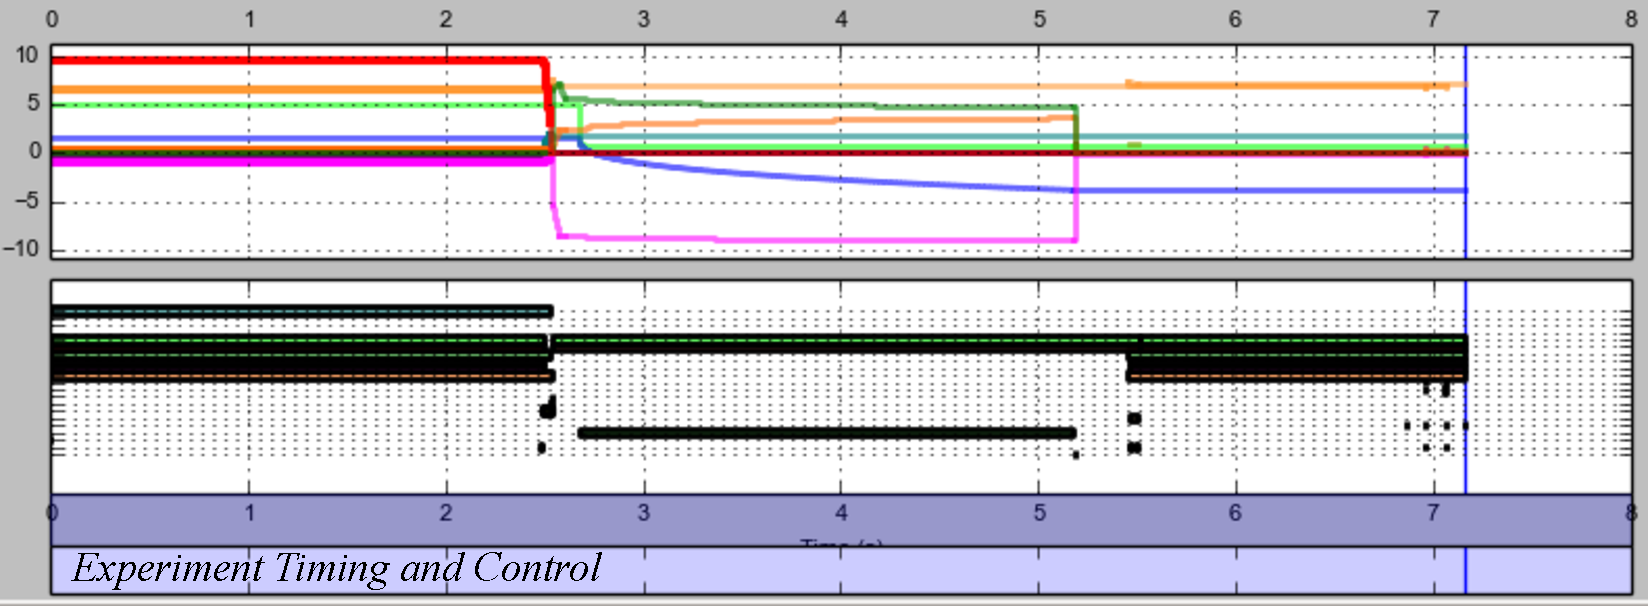
\includegraphics[width=.8\textwidth]{intro/figures/sample-timing}
    }
    \vspace{1em}
    {\Large\rm This Document Last Revised \mandate}
}

\titlepage{\ttitle}
{ %authors
\begin{center}
\begin{Large}
{\hspace{-2em}This Manual Written by:}\\
Dr. Spencer E. Olson$^{\rm a}$\\
Dr. Rudolph N. Kohn$^{\rm b}$
}
{ % address
    $^{\rm a}$ Air Force Research Laboratory \\
    $^{\rm b}$ Space Dynamics Laboratory\\
    \vspace{1em}
    AFRL/RVBY \\
    Battle Space Environment Division \\
    Cold Atom Laboratory \\
    3550 Aberdeen Ave, SE\\
    Kirtland AFB, NM 87117-0001\\
    \href{mailto:afrl.cold-atoms@us.af.mil}{afrl.cold-atoms@us.af.mil}
\end{Large}
\end{center}
}

%\thispagestyle{fancy}

\initializefrontsections

\pagestyle{fancy}

% Copyright page
%\unnumberedpage
%\copyrightpage{%
%--All\ Goverment\ Rights\ Granted%
%}

\setcounter{page}{1}



% Table of contents, list of figures, etc.
\setcounter{tocdepth}{3}
\setcounter{secnumdepth}{3}
\tableofcontents
\listoftables
\listoffigures
\printgloss[symb]{symbols} % list of symbols
\listofappendices


\startthechapters 
\normalsize
% use chapter command:
% usage:  \newchapter{Title}{sub-directory}{tex-file}
% tex-file is relative to sub-directory/ and should not have the .tex ending.
%\def\suppressbibtoc{1}
\newchapter{Introduction}{intro}{intro}
\newchapter{Installation}{install}{install}
\newchapter{Quick Start}{quickstart}{quickstart}
\newchapter{Operational Overview}{op-overview}{overview}
\newchapter{Device Configuration}{devcfg}{devcfg}
\newchapter{Channel Configuration}{channels}{channels}
\newchapter{Waveforms}{waveforms}{waveforms}
\newchapter{Iterating}{iterating}{iterating}
\newchapter{Scripting}{scripting}{scripting}


\startappendices
\newappendix{Arbwave Version Rules}{versions}{versions}
\clearpage
\vspace*{\fill}
\centerline{This page intentionally left blank}
\vspace*{\fill}


% Index and Bibliography in single spacing
\linespread{1.0}
\selectfont

% Print Acronyms
\section*{}
\printgloss[acro]{acronyms}

% Print the index
%\clearpage
\section*{}
\addcontentsline{toc}{chapter}{Index}
\printindex
%\clearpage


% Print the Bibliography
%\def\suppressbibtoc{0}
\section*{}\nopagebreak
\addcontentsline{toc}{chapter}{BIBLIOGRAPHY}
\bibliography{manual}

\end{document}

